% !TEX program = xelatex
\documentclass[10pt, a4paper]{article}
\usepackage{extarrows} 
% ===== Essential Packages =====
\usepackage[T1]{fontenc}          % Better font encoding
\usepackage{lmodern}              % Modern Latin Modern font
\usepackage[UTF8, fontset=none]{ctex}  % Chinese support, no preset fontset
\usepackage{xeCJK}                % XeCJK for better font control

% Set CJK fonts (using fonts available on your system)
\setCJKmainfont{Noto Serif CJK SC}    % Main Chinese font
\setCJKsansfont{Noto Sans CJK SC}     % Sans-serif Chinese font
\setCJKmonofont{Noto Sans Mono CJK SC} % Monospace Chinese font

% ===== Math & Symbols =====
\usepackage{amsmath}              % Advanced math
\usepackage{amssymb}              % Additional math symbols
\usepackage{mathrsfs}             % Ralph Smith's Formal Script
\usepackage{braket}               % Dirac bra-ket notation

% ===== Graphics & Tables =====
\usepackage{graphicx}             % Image support
\usepackage{float}                % Better float control
\usepackage{wrapfig}              % Wrapped figures
\usepackage{tikz}                 % Vector graphics
\usepackage[table]{xcolor}        % Colored tables
\usepackage{array}                % Enhanced tables
\usepackage{multirow}             % Multirow tables
\usepackage{tabularx}             % Adjustable-width tables
\usepackage{booktabs}             % Professional table lines
\usepackage{siunitx}              % SI units in tables
\usepackage{caption}              % Better captions
\usepackage{subcaption}           % Sub-captions
\usepackage{adjustbox}            % Box resizing

% ===== Code Listings =====
\usepackage{listings}             % Code blocks
\usepackage{tcolorbox}            % Colored boxes
\tcbuselibrary{listings, breakable} % Listings in tcolorbox

% ===== Misc =====
\usepackage{lipsum}               % Dummy text
\usepackage{footmisc}             % Better footnotes
\usepackage[margin=1in]{geometry} % Page margins
\usepackage{diagbox}
\usepackage{mathtools}
\usepackage{tensor}
\lstset{
	basicstyle=\small\ttfamily,
	numbers=left,
	numberstyle=\tiny\color{gray},
	keywordstyle=\color{blue},
	commentstyle=\color{green!60!black},
	stringstyle=\color{red},
	frame=single,
	breaklines=true,
	showstringspaces=false,
	tabsize=2,
	captionpos=b
}
\author{
	张世航 \\
	学号:320230938701 \\
	\texttt{zhshihang2023@lzu.edu.cn}
}
\title{光纤光栅}

\begin{document}
	\maketitle
	\section{波长随温度的变化}
     \begin{figure}[H]
		\centering
		
\includegraphics[width=0.5\linewidth]{1.pdf}
		\label{fig:1}
	\end{figure}
    我们知道
    \begin{equation}
        \frac{\Delta \lambda_B}{\lambda_B} = \alpha\Delta T\rightarrow \frac{\Delta \lambda_B}{\Delta T}=\alpha \lambda_B=0.0102nm/K
    \end{equation}
    \begin{equation}
        \alpha = \frac{0.0102nm/K}{\bar{\lambda}_B}=6.601090577570692\times 10^{-6}1/K
    \end{equation}

    \section{波长随拉力的变化}
    \begin{equation}
        \frac{\Delta\lambda_B}{\lambda_B} = (1-P_e)\epsilon = 0.22k\Delta G
    \end{equation}
    \subsection{拉力增大的过程}
    \begin{figure}[H]
		\centering
		
\includegraphics[width=0.5\linewidth]{2.pdf}
		\label{fig:2}
	\end{figure}
    \subsection{拉力减小的过程}
    \begin{figure}[H]
		\centering
		
\includegraphics[width=0.5\linewidth]{3.pdf}
		\label{fig:3}
	\end{figure}
    \begin{equation}
        \frac{\Delta \lambda_B}{\Delta G} = 0.22k \lambda_B=0.0012nm/N
    \end{equation}

    \begin{equation}
        k=\frac{0.0012nm/N}{0.22\lambda_B} = 3.515270383368553\times 10^{-6}1/N
    \end{equation}

    我们回到波长和质量的关系,画出关系图
    \begin{figure}[H]
		\centering
		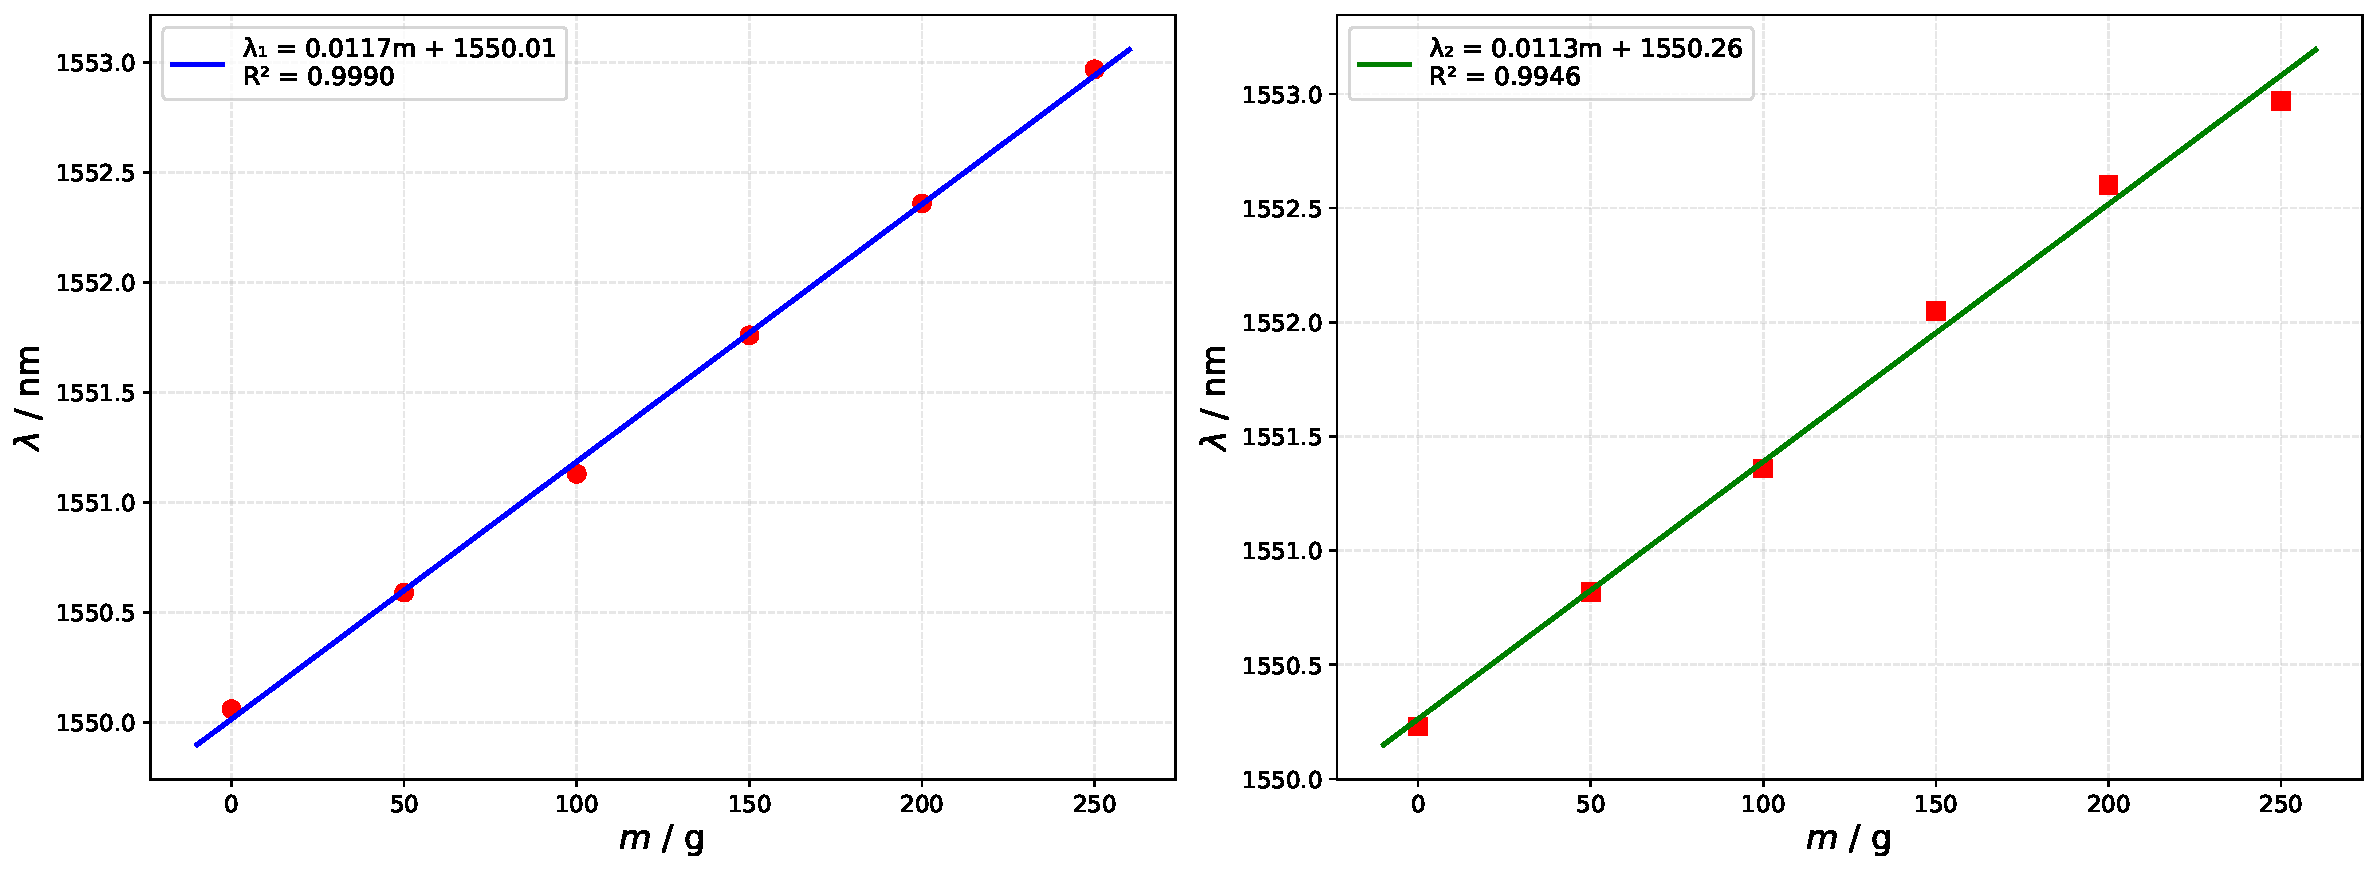
\includegraphics[width=0.5\linewidth]{combined_fit.pdf}
		\label{fig:4}
	\end{figure}
    \begin{figure}[H]
		\centering
		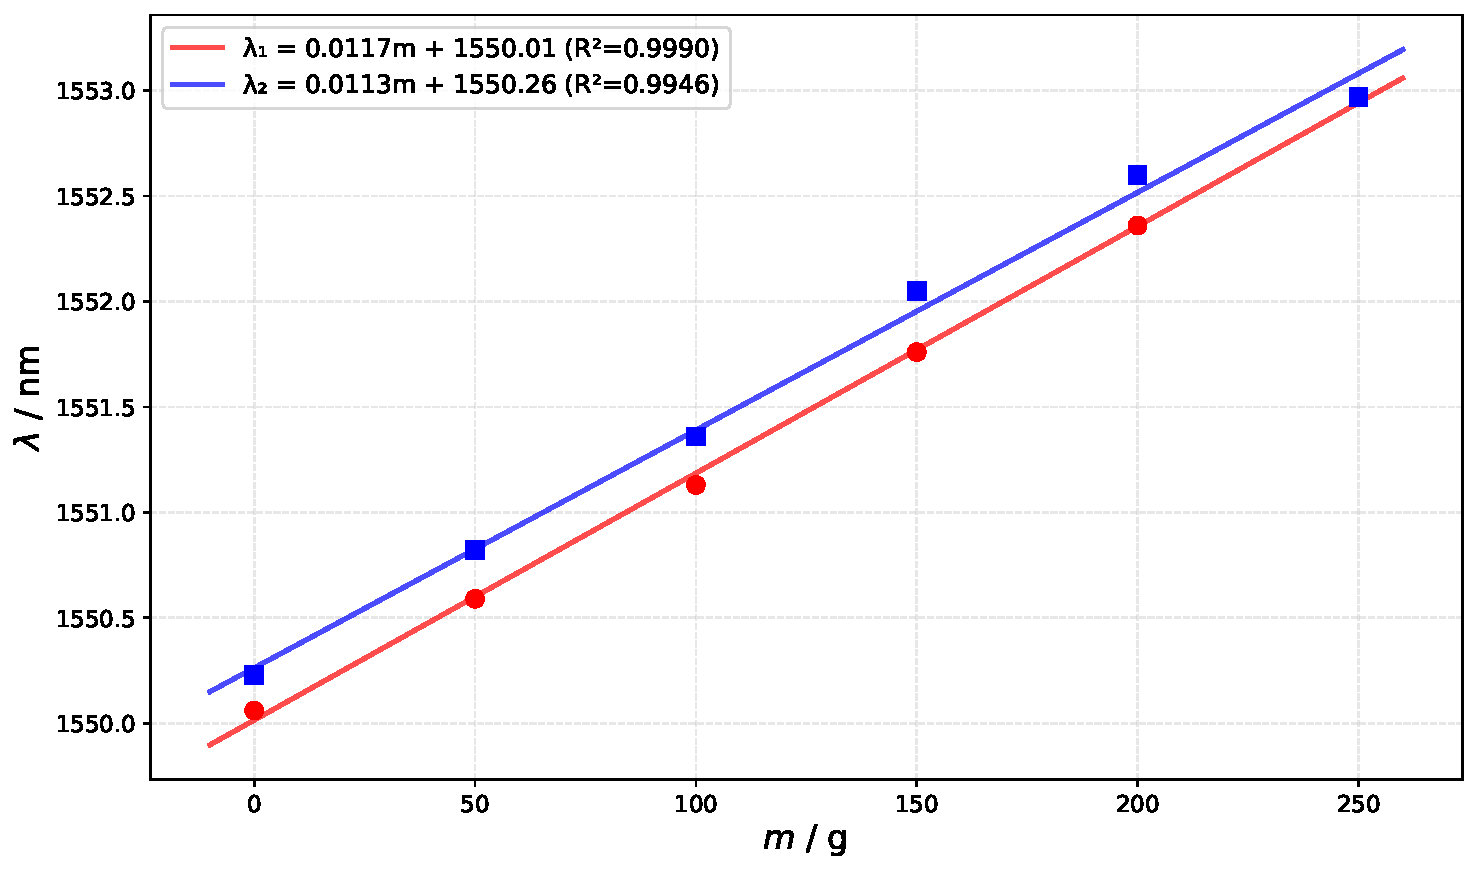
\includegraphics[width=0.5\linewidth]{overlay_fit.pdf}
		\label{fig:5}
        \caption{红色的线是拉力增大的曲线,蓝色的线是拉力减小的曲线}
	\end{figure}
\end{document}